\section{Unity} \label{unity}

Unity è una Game Engine (GE) cross-platform sviluppata da Unity Technologies, utilizzata per la creazione di videogiochi (sia 2D che 3D) e simulazioni, che supporta la distribuzione su una larga varietà di piattaforme (PC, console, dispositivi mobili, etc.). Fornisce astrazioni che contribuiscono ad estendere il suo utilizzo tra gli sviluppatori e programmatori, rendendola una delle GE più utilizzate per produrre in maniera veloce ed efficace applicazioni e giochi.\cite{unity}

\medskip

Inoltre, questa GE supporta molte funzionalità facili da utilizzare e sfruttabili per creare giochi realistici e simulazioni immersive, come un intuitivo editor real-time, un sistema di fisica integrato, luci dinamiche, la possibilità di creare oggetti 2D e 3D (direttamente dall'IDE o di importarli esternamente), gli shader, un supporto per l'intelligenza artificiale (capacità di evitare gli ostacoli, ricerca del percorso, etc.), e cosi via.

\medskip

Le funzionalità principali messe a disposizione del designer sono:
\begin{itemize}
	\item \textbf{GameObject}: La classe base per tutte le entità presenti su una scena di Unity- un personaggio controllabile dall'utente, un personaggio non giocabile, un oggetto (2D/3D). Tutto ciò che è presente sulla scena è dunque un GameObject.
	\item \textbf{Script}: Il codice sorgente applicato a un GameObject, grazie al quale è possibile assegnare a quest'ultimo comportamenti e proprietà dinamiche. Gli script vengono eseguiti dal game loop di Unity che, in maniera sequenziale, esegue una volta ogni script durante ogni frame del gioco. Non esiste concorrenza. Il comportamento è il risultato della logica definita nello script attraverso funzioni e routine. Le proprietà equivalgono a variabili che possono essere valorizzare nello script oppure definite dall'IDE grafico.
	\item \textbf{Component}: Elemento, proprietà speciale assegnabile ai GameObject. A seconda del tipo di GameObject che si desidera creare è necessario aggiungere diverse combinazioni di Component. I Component basilari riguardano la fisica (Transform, Collider,..), l'illuminazione (Light) e la renderizzazione del GameObject (Render). \'E possibile istanziare runtime Components attraverso gli script.
	\item \textbf{Coroutine}: Una soluzione alla sequenzialità imposta agli script, grazie al quale è possibile partizionare una computazione e distribuirla su più frame, sospendendo e riprendendo l'esecuzione in precisi punti del codice.
	\item \textbf{Prefab}: Rappresentazione di un GameObject complesso, completo di Script e Component, istanziabile più volte runtime. Le modifiche della struttura, le proprietà ed i componenti del Prefab si propagheranno a tutti i GameObject collegati allo stesso presenti nella scena di gioco.
	\item \textbf{Event e Messaging System}: sistema ad eventi utile per far comunicare tra loro diversi GameObject. Questi sistemi sono formati tipicamente da eventi e listener. I listener si sottoscrivono ad eventi di un certo tipo: quando l'evento si verifica, viene notificato a tutti i listener dello stesso tipo che sono in ascolto attraverso l'invio di un messaggio.
\end{itemize}

\section{Realizzare un ambiente in Unity} \label{ambiente_unity}

Gli strumenti a disposizione in Unity mettono nelle mani degli sviluppatori la possibilità di realizzare qualunque tipo di oggetto: dai più semplici, come un cubo, ai più articolati, ad esempio un robot. 

\medskip

Per realizzare oggetti complessi è possibile creare una gerarchia di componenti e dotare ognuno di loro delle stesse funzionalità dell'oggetto padre. Ripensando all'esempio del robot, lo sviluppatore può suddividere lo stesso in sotto-componenti più articolate, quali testa, braccia, addome, gambe, fino ad arrivare a realizzare parti basilari quali dita, occhi e così via.

\medskip

Successivamente alla realizzazione dello scheletro dell'oggetto, attraverso la definizione di "script" e l'associazione di "components" è possibile animarlo, dargli una specifica fisicità e renderlo consapevole dell'ambiente che lo circonda. Verranno ora fatti degli esempi per ognuna delle funzionalità appena descritte.

\begin{figure}[H]
\centering
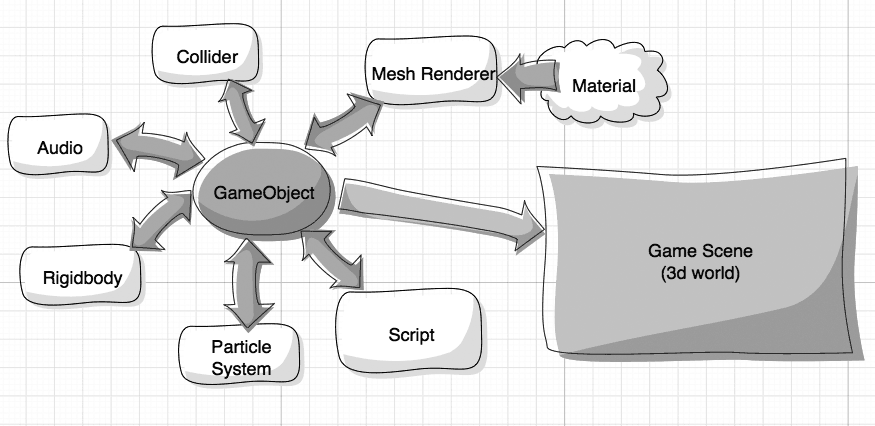
\includegraphics[width=\textwidth]{figures/unity_diagram.png}
\caption{GameObject e Components}
\end{figure}

\subsection{Muovere un GameObject}

Come spiegato precedentemente, ogni oggetto presente su Unity è un GameObject e, per definizione, contiene le seguenti proprietà fondamentali: 
\begin{itemize}
    \item Posizione
    \item Scala
    \item Rotazione
\end{itemize}
Le proprietà appena elencate sono elementi fondamentali del "component" Transform \cite{unity_transform}, il quale viene automaticamente realizzato per ogni oggetto in scena.

\medskip

Attraverso l'associazione con uno script, lo sviluppatore può accedere ad ogni proprietà del GameObject. In tal modo è possibile modificare runtime la sua posizione, la scala e la rotazione e, applicando diverse tipologie di trasformazioni, lo si anima. Questa modalità di animazione è basilare, ma sufficiente per l'obiettivo finale posto. Sono poi presenti meccanismi complessi in caso di elaborazioni più articolate e specifiche come, ad esempio, la simulazione della corsa umana.

\subsection{Fisicità del GameObject}

La semplicità nella realizzazione di oggetti all'interno delle Game Engine è affiancata alla presenza di un motore fisico: attraverso quest'ultimo, l'IDE elabora e modifica dinamicamente ogni oggetto in scena in base alle specifiche fisiche ad esso attribuite. Il motore fisico rende possibile la simulazione di forza di gravità, la fisica dei movimenti e le occlusioni della scena.

\medskip

In Unity, per definire la fisicità di un GameObject, è necessario attribuirgli uno specifico "component" chiamato RigidBody \cite{unity_rigidbody}. Aggiungendo questo componente, il movimento del GameObject nella scena è controllato dal motore fisico di Unity. Di questo componente è possibile specificare:
\begin{itemize}
    \item Massa
    \item Resistenza
    \item Velocità di movimento
    \item Soggezione alla gravità
\end{itemize}

\subsection{Percepire l'ambiente}

La percezione generalmente è associata all'acquisizione di una realtà interna o esterna attraverso l'elaborazione organica e psichica di stimoli sensoriali \cite{treccani}. Nelle Game Engine, rendere un oggetto capace di percepire la realtà è spesso collegato a renderlo fisicamente consapevole della propria superficie.

\medskip

Su Unity è presente il "Collision Detection System", il quale controlla ogni evento di interazione fisica tra due o più GameObject nella scena e, attraverso l'aggiunta del "component" Collider al GameObject, viene specificato che l'oggetto deve essere preso in considerazione dal sistema durante questi eventi.

\medskip

Il Collider è associabile ad un GameObject, più o meno complesso, ed è capace di creare un'area generica, come ad esempio un cubo/sfera, che circonda l'oggetto, oppure mappare alla perfezione la sua superficie. Gli eventi di interazione creati dal "Collision Detection System" sono utilizzabili, da parte dello sviluppatore, nello script collegato al GameObject, difatti durante una collisione vengono invocati degli specifici metodi all'interno dello script con tutte le informazioni sull'evento. \cite{unity_collision}

L'ultimo passaggio è fondamentale, dato che permette di completare il processo di percezione dell'ambiente da parte di un generico GameObject e, quindi, lo rende consapevole della propria presenza nella scena.

\medskip

Per aumentare la capacità di percezione del GameObject, all'interno di Unity ogni oggetto può essere visto e utilizzato da ogni altro oggetto in scena. In questa maniera oltre alla percezione del proprio corpo fisico, il GameObject è in grado di conoscere anche quali altri elementi compongono la scena, ottenendo quindi la percezione totale dell'ambiente.

\medskip

Tutte le procedure sopra illustrate sono replicabili per ogni GameObject presente in scena. In questo modo è possibile realizzare scene più o meno complesse.

\subsection{Modificare l'ambiente}

Il GameObject, come illustrato in precedenza, è la classe base di tutti gli oggetti presenti su una scena Unity, di conseguenza, l'ambiente stesso è un GameObject (più o meno complesso). Questo concetto, unito alla possibilità di ogni GameObject di interagire sia fisicamente che logicamente (script) con ogni altro oggetto in scena, dà luogo ad infinite possibilità di modifica della scena. Ad esempio, in caso di collisione tra due oggetti, il motore fisico, unito al motore grafico, calcola il possibile spostamento degli stessi che quindi porta ad un'effettiva modifica dell'ambiente.

\section{Unity come ambiente in un MAS}

L'ambiente all'interno di un MAS è catalogato come "contenitore" in cui gli agenti sono immersi e con il quale questi ultimi possono interagire, modificandolo. La caratteristica degli agenti di essere situati nell'ambiente in cui si trovano permette loro di percepire e produrre cambiamenti su di esso. Con le procedure sopra descritte è dunque possibile modellare l'ambiente da un punto di vista fisico e, quindi, dare un corpo agli agenti e se necessario anche agli artefatti. Di conseguenza, possedendo un corpo fisico (GameObject) ogni agente e/o artefatto è effettivamente in grado di produrre cambiamenti nella scena e quindi modificare l'ambiente.
